\documentclass[UTF8,12pt,a4paper,oneside]{ctexbook}
\usepackage[left=3.0cm,right=2.0cm,top=3.0cm,bottom=2.5cm]{geometry}
\usepackage{setspace}
\usepackage{hyperref}
\hypersetup{hidelinks}
\usepackage{booktabs}
\usepackage{array}
\usepackage{graphicx}
\usepackage{pdfpages}
\usepackage{amsmath}
\usepackage{float}
\usepackage{needspace}
\usepackage{caption}
\usepackage{fancyhdr}
\usepackage{makecell}
\usepackage{titlesec}
\usepackage{chngcntr}
\usepackage{etoolbox}
\usepackage{tikz}
\usetikzlibrary{arrows.meta,positioning,shadows.blur}
\usepackage[backend=biber,style=gb7714-2015]{biblatex}
\addbibresource{refs.bib}
\AtBeginBibliography{\sloppy}
\setstretch{1.5}
\setmainfont{Times New Roman}
\setCJKmainfont{SimSun}[BoldFont=SimSun,BoldFeatures={FakeBold=2}]
\setCJKsansfont{Microsoft YaHei}
\setCJKmonofont{FangSong}
% 使用 ctex 内置黑体命令，避免系统字体兼容问题
\setCJKfamilyfont{song}{SimSun}[BoldFont=SimSun,BoldFeatures={FakeBold=2}]
\xeCJKsetup{AutoFakeBold=true}
\ctexset{
  chapter={
    name={,},
    number=\arabic{chapter},
    format=\heiti\zihao{3},
    beforeskip=0pt,
    afterskip=1.0\baselineskip
  },
  section={
    format=\heiti\zihao{-4},
    beforeskip=0.5\baselineskip,
    afterskip=0.5\baselineskip
  },
  subsection={
    format=\heiti\zihao{-4},
    beforeskip=0.5\baselineskip,
    afterskip=0.5\baselineskip
  }
}
\captionsetup[table]{font={small,bf},labelfont={bf},labelsep=space,justification=centering,singlelinecheck=true}
\captionsetup[figure]{font={small},labelfont={normalfont},labelsep=space,justification=centering,singlelinecheck=true}
\captionsetup{compatibility=false}
\setlength{\abovecaptionskip}{6pt}
\setlength{\belowcaptionskip}{4pt}
\setlength{\headheight}{15pt}
\setlength{\emergencystretch}{8em}
\setlength{\parindent}{2em}
\fancyhf{}
\fancyfoot[R]{\rmfamily\fontsize{9pt}{9pt}\selectfont\thepage}
\renewcommand{\headrulewidth}{0pt}
\renewcommand{\footrulewidth}{0pt}
\renewcommand{\arraystretch}{1.15}
\raggedbottom
\AtBeginDocument{\zihao{-4}}
% 正文层级“款、项”格式：1、 和 (1)
\newcommand{\kuan}[1]{\par\noindent\CJKfamily{song}\zihao{-4}#1、}
\newcommand{\xiang}[1]{\par\noindent\hspace*{2em}\CJKfamily{song}\zihao{-4}(#1)}
\numberwithin{equation}{chapter}
\counterwithin{figure}{chapter}
\counterwithin{table}{chapter}
\renewcommand{\thefigure}{\thechapter.\arabic{figure}}
\renewcommand{\thetable}{\thechapter.\arabic{table}}
\newcommand{\figref}[1]{图~\ref{#1}}
\newcommand{\tabref}[1]{表~\ref{#1}}
\newcommand{\eqreftext}[1]{见式~\eqref{#1}}
\newcommand{\captab}[1]{表~#1}
\newcommand{\capfig}[1]{图~#1}
\newcommand{\thesisfig}[2]{%
  \IfFileExists{#1}{%
    \includegraphics[width=#2\textwidth]{#1}%
  }{%
    \fbox{%
      \parbox[c][0.28\textheight][c]{#2\textwidth}{\centering
      待插入图片\\[4pt]\texttt{\detokenize{#1}}}%
    }%
  }%
}
\newcommand{\thesisfigfit}[3]{%
  \IfFileExists{#1}{%
    \includegraphics[width=#2\textwidth,height=#3\textheight,keepaspectratio]{#1}%
  }{%
    \fbox{%
      \parbox[c][#3\textheight][c]{#2\textwidth}{\centering
      待插入图片\\[4pt]\texttt{\detokenize{#1}}}%
    }%
  }%
}

\title{家用安防与智能家居联动系统设计}
\author{作者姓名}
\date{\today}

\begin{document}

\pagestyle{empty}
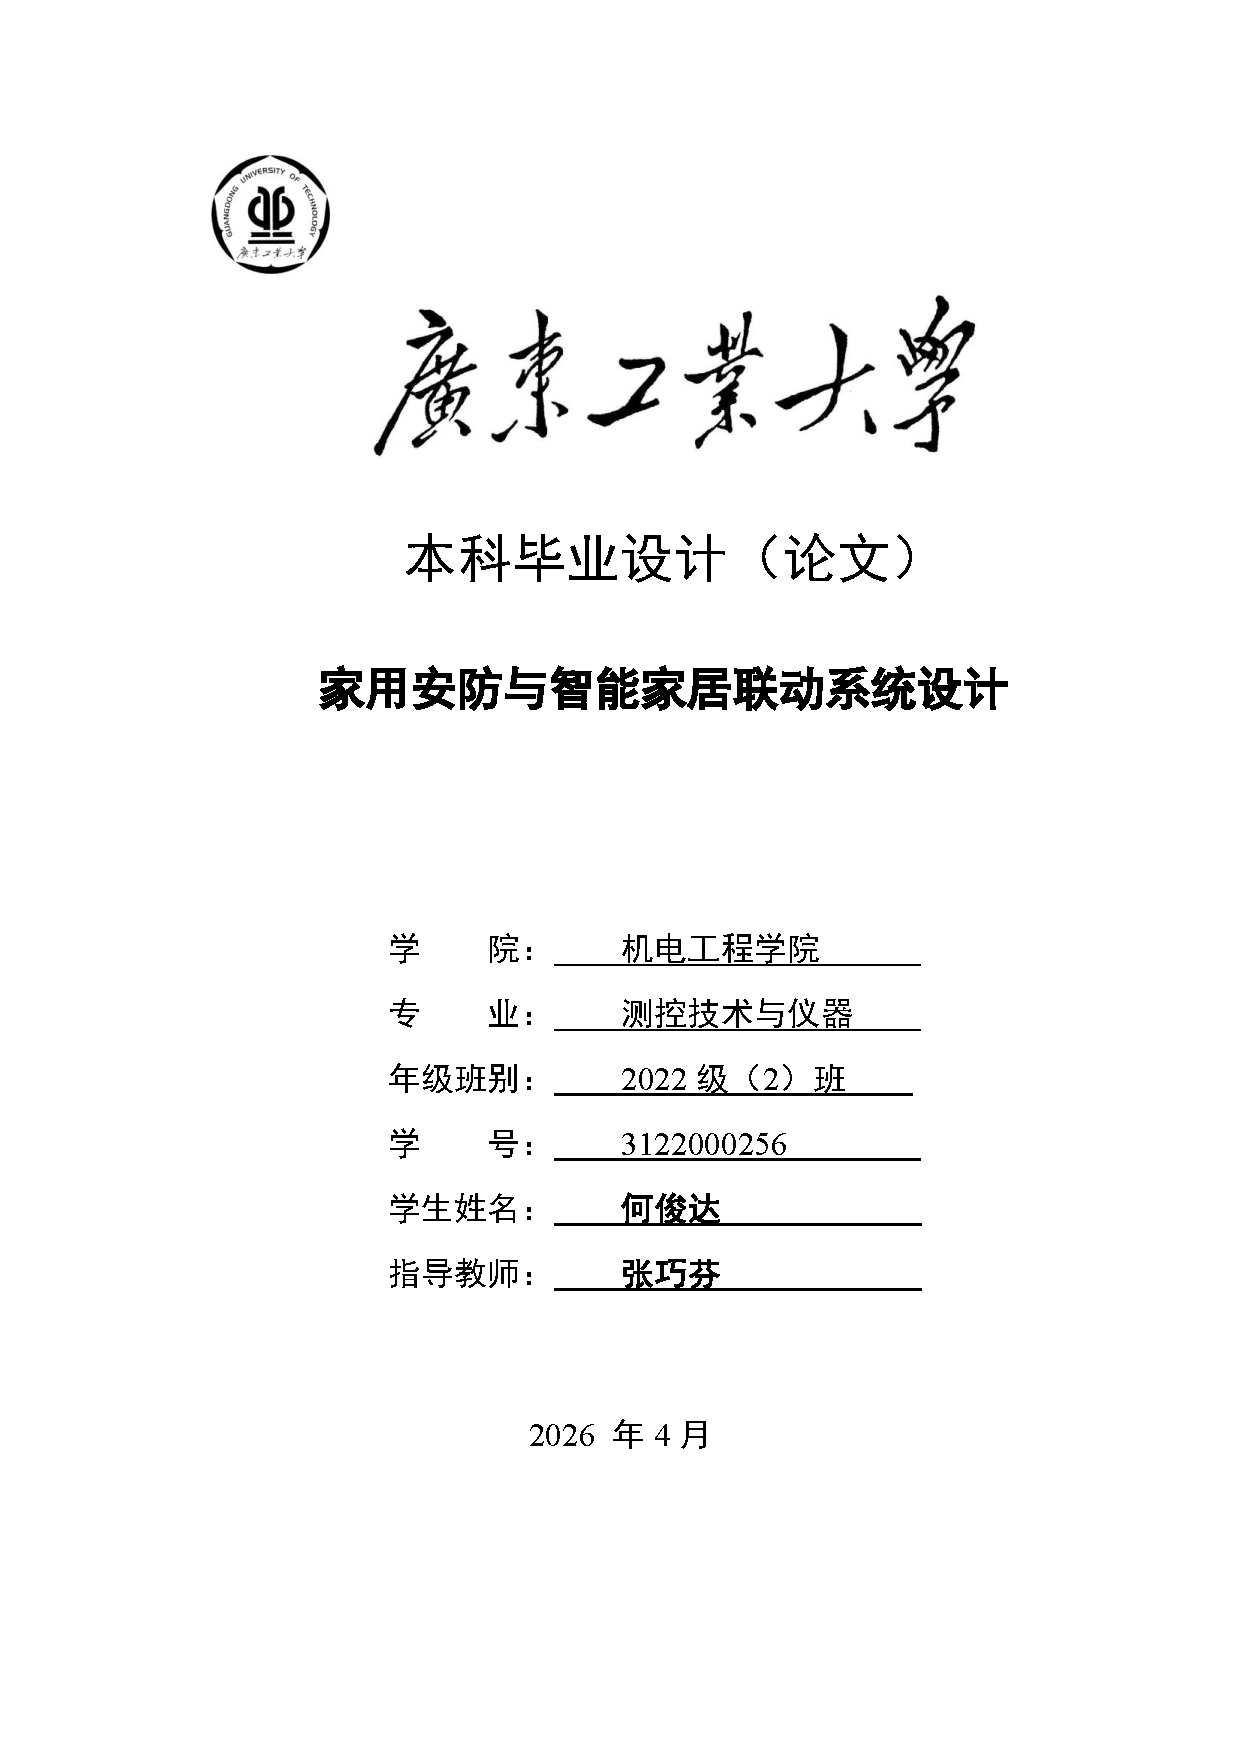
\includepdf[pages=1,pagecommand={},fitpaper=true]{../规范与封面/论文封面.pdf}

\frontmatter
\pagenumbering{gobble}
\tableofcontents
\clearpage

\chapter*{摘要}
\addcontentsline{toc}{chapter}{摘要}
\begin{center}
{\heiti\zihao{3}摘要}
\end{center}
这几年家庭场景对安防、环境监测和远程控制的要求明显提高，传统只做单点报警的设备已经不太够用。结合本课题工程实现过程，本文围绕家用安防与智能家居联动系统展开设计与验证，给出一套基于单芯片STM32F103RCT6的软硬件一体化方案，重点解决设备协同不足、关键流程闭环不完整和异常场景处理能力偏弱等问题。

硬件侧集成AS608指纹识别、PIR红外检测、DHT温湿度采集、MQ-2气体传感、OV7670+FIFO本地抓拍、SD卡存储以及门锁/燃气阀/蜂鸣器执行单元，构成“感知-判定-执行-反馈”的本地自治闭环。软件侧采用“裸机调试模式+FreeRTOS运行模式”可切换架构，通过任务分层和事件驱动实现门禁认证、布撤防控制、入侵告警、燃气应急处置、日志记录与串口JSON状态输出。通信侧由ESP8266（USART3）接入OneNET MQTT通道，支持状态上报、命令下发与远程协同控制；安全侧在本地存储与传输链路中分别引入AES与TLS能力，提升系统安全性和工程可用性。

系统验证按“单元功能-场景联动-性能指标-稳定性”四个层次开展。结果显示，系统在典型家庭场景下能够稳定实现本地自治闭环与远程协同控制，关键链路响应达到预设要求，核心功能完成率较高且结果可重复；连续运行测试中系统也表现出较好的稳定性和容错恢复能力。总体来看，单芯片集中控制方案在毕业设计规模下可以较好平衡实现复杂度、调试效率与后续扩展空间，可为低成本、可复用的家庭安防联动系统提供可落地的工程参考。

\vspace{1\baselineskip}
\noindent{\heiti\zihao{4}关键词}\,\zihao{-4}智能家居，家庭安防，STM32F103RCT6，FreeRTOS，MQTT

\vspace{0.5\baselineskip}
\noindent{\heiti\zihao{4}课题来源}\,\zihao{-4}企、事业单位委托项目

\clearpage
\addcontentsline{toc}{chapter}{英文摘要}
\begin{center}
{\bfseries\zihao{3}Abstract}
\end{center}
\begin{sloppypar}
With increasing demands for integrated home protection, environment awareness, and remote interaction, traditional isolated security devices are no longer sufficient for practical household scenarios. This thesis investigates and implements a home security and smart home linkage system based on a practical engineering implementation, and proposes an integrated hardware-software solution centered on a single-chip STM32F103RCT6 architecture.

At the hardware level, the system integrates AS608 fingerprint access, PIR intrusion sensing, DHT temperature-humidity acquisition, MQ-2 gas monitoring, OV7670+FIFO local image capture, SD-card storage, and actuator modules for door lock, gas valve, and buzzer, forming a local closed-loop chain of sensing, decision, execution, and feedback. At the software level, a switchable architecture between bare-metal debugging mode and FreeRTOS runtime mode is designed to support access control, arming/disarming, intrusion alarm, gas emergency response, logging, and serial JSON status output. For networking, ESP8266 over USART3 connects to OneNET MQTT services for telemetry upload and remote command interaction. Security enhancement is implemented through AES-based local sensitive data protection and optional TLS-secured communication paths.

System validation follows a layered test strategy covering unit function, scenario linkage, performance metrics, and long-term stability. Results show that the prototype reliably supports both local autonomous protection and remote collaborative control in representative household conditions, while maintaining expected response behavior on critical paths and stable operation in continuous tests. The study demonstrates that a single-controller design can balance implementation complexity, debugging efficiency, and extensibility at undergraduate project scale, and provides a practical engineering reference for low-cost, reusable home security linkage systems.
\end{sloppypar}

\vspace{1\baselineskip}
\noindent{\bfseries\zihao{4}Key words}\,smart home，home security，STM32F103RCT6，FreeRTOS，MQTT

\mainmatter
\pagestyle{fancy}
\fancyhf{}
\fancyfoot[R]{\rmfamily\fontsize{9pt}{9pt}\selectfont\thepage}
\renewcommand{\headrulewidth}{0pt}
\renewcommand{\footrulewidth}{0pt}
\setcounter{page}{1}

\chapter{绪论}
\section{研究背景与意义}
随着物联网、嵌入式系统与移动互联网技术的快速发展，智能家居逐步由单设备自动化向多设备协同联动演进\cite{smart_home_survey_2017,home_security_iot_2020}。传统家庭安防系统通常存在功能割裂、联动能力不足与远程管理能力有限等问题，难以满足用户对实时性、可靠性与便捷性的综合需求。在家庭安全事件中，门禁失效、入侵行为、燃气泄漏与环境异常往往具有突发性与并发性，要求系统具备快速感知、准确判断与及时执行能力。

本课题面向家庭实际场景，构建家用安防与智能家居联动系统，研究多源传感感知、单芯片多任务控制、网络通信与安全机制等关键技术。课题研究意义体现在三个方面：其一，提升家庭安防系统的智能化与联动化水平；其二，验证单芯片STM32平台在多外设并发场景下的工程可行性；其三，为低成本、可扩展的家居安防方案提供可复用的设计参考。

从工程应用看，家庭安防系统的价值不只在“发现风险”，更在“资源有限时也能稳定把风险处理好”。本研究在方案设计时抓住三点：本地自治闭环优先，保证断网时还有最小可用能力；链路分层解耦，减少感知、决策、执行和通信之间的连带影响；可维护性优先，通过模块化接口和可配置参数降低后期调试成本。这三点贯穿硬件选型、软件架构和测试验证全过程，让系统不只是能做出来，也能稳定跑起来。
\section{国内外研究现状}
国外在家庭安防与智能家居领域起步更早，已经形成以云平台为核心的生态体系，低功耗广域接入、轻量网关、语音交互和多模态身份认证都比较成熟\cite{smart_home_survey_2017,bozorgi2026_iot_arch,serepas2025_gateway,alkanan2026_biometric}。这类方案普遍强调标准化协议和平台化部署，设备互联和用户体验做得较完整；面向家庭场景的自动漏洞扫描与风险优先级研究也在持续推进\cite{rivas2026_vulnerability}。但有些方案仍依赖私有生态和订阅服务，在本地自治、成本控制和二次开发方面还有约束。

国内相关研究和产业应用发展很快，围绕STM32主控、环境监测、云平台接入、移动端交互和联动控制已经形成较完整的应用链\cite{lian2025_trend,wang2024_stm32_linkage,yue2022_stm32_iot_home,cai2023_stm32f103_control}。近几年高校研究继续拓展到多协议融合、OneNET平台协同、ZigBee组网、远程安防和固件安全分析\cite{wang2024_home_security_wireless,ji2024_stm32_zigbee,chen2023_onenet_ai,zhang2022_firmware_security}，在气体泄漏监测和家庭安全联动方面也给出了较多可行案例\cite{yusuf2026_gas_leakage,dong2024_env_monitor}。不过从工程落地看，异构设备兼容、控制逻辑整合、通信安全和异常容错仍是常见短板，这也是本文继续做一体化联动设计的现实动因。
\section{研究目标与主要内容}
本研究的总体目标是设计并实现一套具备“感知-决策-执行-反馈”闭环能力的家用安防与智能家居联动系统，实现门禁验证、入侵预警、环境监测、燃气应急与远程协同控制等核心功能，并在保障系统实时性的基础上提升数据安全性与系统鲁棒性。

围绕上述目标，论文主要做了六项工作：完成系统需求分析与总体方案设计，确定四层架构和单芯片控制模式；完成硬件选型与电路实现，集成指纹、红外、温湿度、气体和图像采集模块；构建可在裸机与FreeRTOS间切换的软件框架；设计本地串口调试与ESP8266-MQTT远程通信机制；实现AES-128本地安全存储并预留TLS链路扩展能力；通过系统化测试验证功能完整性与工程可运行性。

为保证研究工作具备可复现性与可评价性，论文同时给出量化评价口径：以识别准确率、误报率、关键路径时延、远程协同控制成功率和连续运行稳定性作为核心指标，并通过多轮重复测试降低偶然因素影响。该评价体系与工程目标一一对应，可用于指导后续版本迭代与方案横向对比。
\section{论文结构安排}
本论文共分为7个章节，各章节的核心内容安排如下：第1章为绪论，阐述课题的研究背景与意义，分析国内外研究现状与现有系统的不足，明确课题的研究目标与主要内容，介绍论文的整体结构安排。第2章为系统总体方案设计，完成系统的需求分析，设计系统的总体架构与单芯片功能划分，规划系统的全链路工作流程，完成关键技术的选型与论证。第3章为系统硬件设计与实现，详细介绍核心控制器最小系统、传感器模块、执行器驱动、摄像头与SD接口、电源管理等硬件电路的设计与实现过程。第4章为系统软件设计与实现，介绍系统的软件开发环境与总体软件架构，详细阐述底层驱动开发、核心控制逻辑、任务机制、网络通信与数据安全机制。第5章为手机端交互与远程控制设计，介绍设备通信主题、状态监控与控制流程。第6章为系统集成测试与性能评估，搭建测试环境，设计测试用例，完成系统的单元测试、联动功能测试、性能指标测试与稳定性测试。第7章为总结与展望，对全文的研究工作进行全面总结，分析系统优势与不足，并给出后续优化方向。

\chapter{系统总体方案设计}
\section{系统需求分析}
系统需求分析是总体方案设计的基础。结合家庭场景中的常见风险与使用习惯，系统需要同时满足门禁安全、入侵告警、环境监测与设备联动控制等需求，并支持本地控制与远程管理双通道操作。为保证系统可落地实现，还需综合考虑成本、功耗、开发周期与后续维护等工程因素。
\subsection{功能需求}
在功能层面，系统应实现用户身份验证、室内人体入侵检测、温湿度与气体状态采集、图像信息采集与存储、继电器设备控制、蜂鸣器报警、远程监控与历史日志查询。系统需具备多事件并发处理能力，支持多种触发条件下的自动联动策略，例如气体超阈值时自动切断燃气并触发本地告警。
\subsection{性能需求}
在性能层面，系统应满足嵌入式场景下的实时性与稳定性要求：关键告警路径响应时延应控制在可接受范围内，传感数据采集与上报应具备较高连续性，门禁识别与执行控制需保证准确率和一致性。系统在长期运行中应具备较好的抗干扰能力，避免频繁误报与漏报。
\subsection{工程约束}
工程实现中需遵循硬件资源受限、供电条件有限与部署环境复杂等约束。主控芯片算力与存储容量有限，要求软件架构具备模块化与轻量化特征；系统布线与安装须兼顾安全性与可维护性；通信方案需在可靠性与成本间平衡，保证系统具备可复制与可扩展能力。
\section{系统总体架构}
系统采用四层架构设计，包括感知层、控制层、通信层与应用层。感知层由AS608、PIR、DHT、MQ-2及OV7670+FIFO模块组成，负责状态采集与事件触发；控制层由单芯片STM32F103RCT6承担，统一完成采集、判定与执行；通信层通过USART与MQTT实现本地调试及远程交互；应用层由OneNET平台与基于\texttt{uni-app}开发的移动端页面构成，提供状态展示与控制入口。四层分工明确，形成自底向上的数据流与自顶向下的控制流。
系统总体结构如图\ref{fig:system_arch}所示。
\begin{figure}[H]
\centering
\thesisfig{images/fig2_1_system_arch.png}{0.96}
\caption{系统总体架构}
\label{fig:system_arch}
\end{figure}
\section{单芯片控制架构设计}
针对多模块并发与任务异构特性，系统采用单芯片集中控制架构。该架构在工程上减少板间互联与协议同步成本，同时通过任务化软件设计维持并发处理能力，满足毕业设计阶段对复杂度与可实现性的平衡要求。
\subsection{功能分工}
单芯片侧统一完成网络通信、数据融合、规则匹配、告警上报与外设驱动控制。门锁/燃气阀/蜂鸣器、PIR/DHT/MQ-2、AS608、OV7670+FIFO与SD均由同一控制器管理，降低了接口边界不一致导致的联调风险。
\subsection{资源分配}
资源分配遵循“高实时逻辑优先、本地安全闭环优先”的原则。入侵判定、门禁控制与燃气应急等关键功能在本地直接执行；联网与上报作为增强能力在后台任务中维护。该分配方式可在网络异常时保持基础安防功能可用。
\section{系统工作流程}
系统工作流程覆盖上电初始化、状态监控、事件处理、联动执行与结果反馈等环节。通过流程化设计，可规范各模块协作顺序，降低边界条件下的状态冲突风险。
\subsection{上电启动流程}
系统上电后首先完成时钟、GPIO、串口、定时器等基础外设初始化，随后按配置进入裸机轮询或FreeRTOS任务调度模式。默认调试配置下优先启用本地门禁与安防路径；全功能模式下再激活采集、通信、控制、抓拍与告警任务，实现完整联动。
\subsection{居家/布防/应急流程}
系统支持居家、布防与应急三类典型运行场景。居家模式下重点保障低干扰使用；布防模式下强化入侵检测与告警策略；应急模式在检测到气体异常或高风险事件时优先执行安全联动动作，包括切断燃气、触发蜂鸣器并上报状态，形成快速闭环处理机制。

系统工作流程如图\ref{fig:system_workflow}所示。
\begin{figure}[H]
\centering
\thesisfigfit{images/fig2_2_workflow.png}{0.84}{0.62}
\caption{系统工作流程}
\label{fig:system_workflow}
\end{figure}
\section{关键技术选型}
技术选型以“满足指标约束、保证工程可落地、兼顾成本与扩展性”为核心原则，围绕控制器算力、系统实时性、通信可靠性与数据安全性四个维度进行方案论证。
为便于对比不同方案在实现复杂度、资源开销与可维护性上的差异，关键技术选型对比如图\ref{fig:selection_matrix}所示。
\begin{figure}[H]
\centering
\vspace{0.2em}
\thesisfigfit{images/fig2_3_selection_matrix.png}{0.88}{0.72}
\caption{关键技术选型矩阵}
\label{fig:selection_matrix}
\end{figure}
\clearpage
\subsection{控制器：STM32F103RCT6}
根据单板多外设设计要求，控制器需满足较多GPIO占用、并口摄像头采集、多路串口通信及定时中断资源并发等约束；同时需兼顾开发生态成熟度与器件可获得性。综合评估后，本设计选择STM32F103RCT6作为控制核心，既能满足当前外设规模，也便于后续功能扩展\cite{stm32_ref,stm32_rm0008}。
\subsection{系统：FreeRTOS}
根据主机软件设计要求，系统调度层需要支持多任务并发、优先级抢占、任务间通信和超时管理，保障告警链路实时响应与通信链路持续稳定。若长期使用纯裸机超循环，功能增加后很容易出现时序耦合重、维护成本高、实时性难控制的问题。基于这一点，本设计在主机端选用FreeRTOS，利用其轻量内核、可裁剪机制和任务同步原语完成并发协同，满足资源受限条件下的实时控制需求\cite{freertos_book,freertos_sched}。
\subsection{通信：MQTT}
根据远程监控与控制设计要求，应用层通信协议需要满足低带宽开销、弱网可用、消息异步分发和跨平台接入能力，并支持状态上报、命令下发与告警推送。对比HTTP轮询等方案后，MQTT在报文体积、连接保持和发布/订阅解耦方面更适合物联网终端场景。基于该对比结果，本设计选择MQTT作为设备与移动端之间的核心通信协议，实现高效稳定的消息交互\cite{mqtt_spec,mqtt_v5}。
\subsection{加密：AES-128、TLS}
根据系统安全设计要求，既要防范设备本地存储泄露风险，也要防范公网传输中的窃听与篡改风险。考虑MCU算力与内存约束，本地加密算法需具备实现成熟、资源开销适中与安全强度可接受等特点；网络传输层需具备身份认证与链路加密能力。基于上述约束，本设计采用AES-128对敏感数据进行本地加密存储，并在MQTT通信链路启用TLS安全传输机制，构建“存储+传输”双层防护体系\cite{aes_fips197,rfc5246,tls_rfc}。

\section{本章小结}
本章完成了系统需求分析、总体架构设计、单芯片控制策略与关键技术选型，明确了系统从感知到执行再到反馈的全流程组织方式。通过四层架构与功能分工设计，系统能够在资源受限条件下兼顾实时性、可维护性与可扩展性；通过对控制器、调度机制、通信协议与安全机制的综合论证，形成了可落地的工程实现方案，为后续硬件与软件实现奠定了基础。

\chapter{系统硬件设计}
\section{硬件总体设计}
硬件总体设计遵循模块化与可维护原则，以单芯片控制核心为中心，向外扩展感知、执行、通信与存储单元。各模块通过标准接口连接，便于后续替换升级与故障定位。硬件布局强调信号完整性与电源稳定性，兼顾体积、成本与抗干扰能力。
硬件总体连接关系如图\ref{fig:hw_block}所示。

\begin{figure}[H]
\centering
\thesisfig{images/fig3_1_hw_block.png}{0.85}
\caption{硬件总体连接框图}
\label{fig:hw_block}
\end{figure}

\begin{table}[htbp]
\centering
\caption{系统硬件模块组成与功能}
\renewcommand{\arraystretch}{1.15}
\begin{tabular}{>{\raggedright\arraybackslash}p{3.0cm} >{\raggedright\arraybackslash}p{4.1cm} >{\raggedright\arraybackslash}p{3.1cm} >{\raggedright\arraybackslash}p{2.8cm}}
\toprule
模块类别 & 核心器件 & 主要功能 & 备注 \\
\midrule
主控模块 & STM32F103RCT6（单芯片） & 任务调度、网络通信、联动决策 & 裸机/FreeRTOS可切换 \\
门禁模块 & AS608 & 指纹采集与身份验证 & UART \\
安防检测模块 & HC-SR501 & 人体移动检测 & GPIO中断 \\
环境监测模块 & DHT11/22、MQ-2 & 温湿度/气体采集 & 周期采样 \\
图像采集模块 & OV7670+FIFO & 异常抓拍与图像缓存 & 并口 \\
执行模块 & 门锁/燃气阀继电器、蜂鸣器 & 设备联动与本地报警 & 驱动隔离 \\
存储模块 & SD卡（SPI2） & 抓拍BMP与容量统计 & FatFs \\
\bottomrule
\end{tabular}
\end{table}
\section{主控最小系统设计}
主控最小系统基于STM32F103RCT6构建，包括时钟电路、复位电路、SWD调试下载接口与基础供电电路。系统采用单板集成方式，减少跨板连接带来的接触不良与协议同步问题，提升联调效率。
主控最小系统原理结构如图\ref{fig:mcu_min_system}所示。

\begin{figure}[H]
\centering
\thesisfig{images/fig3_2_mcu_min_system.png}{0.78}
\caption{主控最小系统原理图}
\label{fig:mcu_min_system}
\end{figure}

\begin{table}[htbp]
\centering
\caption{主控最小系统关键参数}
\renewcommand{\arraystretch}{1.15}
\begin{tabular}{>{\raggedright\arraybackslash}p{3.3cm} >{\raggedright\arraybackslash}p{2.9cm} >{\raggedright\arraybackslash}p{6.4cm}}
\toprule
参数项 & 配置 & 说明 \\
\midrule
系统时钟 & 72MHz & 外部晶振+PLL \\
工作电压 & 3.3V & 稳压供电 \\
下载调试接口 & SWD（PA13/PA14） & 关闭JTAG，保留SWD \\
主要串口 & USART1 + USART3 & USART1用于AS608/调试，USART3用于ESP8266 \\
核心外设占用 & OV并口+SPI2+多GPIO & 支持摄像头、SD、传感与执行器并发 \\
\bottomrule
\end{tabular}
\end{table}
\section{感知层模块设计}
感知层承担多源信息采集任务，是系统实现智能判断的基础。各传感模块依据其信号特征与时序要求进行独立驱动设计，并在单芯片内部完成数据融合与事件触发，再通过串口JSON或MQTT进行上报\cite{as608_manual,hcsr501_datasheet,dht22_datasheet,mq2_datasheet,ov7670_datasheet}。
感知层各传感器接线关系如图\ref{fig:sensor_wiring}所示。

\begin{figure}[H]
\centering
\thesisfig{images/fig3_3_sensor_wiring.png}{0.78}
\caption{传感器模块接线示意}
\label{fig:sensor_wiring}
\end{figure}
\Needspace{6\baselineskip}
\subsection{AS608指纹模块}
根据家庭门禁设计要求，身份识别模块需满足较高识别准确率、较短响应时间、较低误识率以及稳定的串口通信能力；在工程实现上需兼顾3.3V系统兼容性、模块体积与集成复杂度。综合比较光学与电容式方案后，优先采用成熟度较高的光学指纹识别模块，要求支持指纹模板管理、1:N检索和快速比对。结合模块标称参数与系统联调需求，本设计选择AS608作为门禁身份识别模块，其供电范围与串口接口便于与STM32平台直接对接，适合长期在线门禁场景\cite{as608_manual}。
\Needspace{6\baselineskip}
\subsection{HC-SR501人体红外}
根据安防布防场景设计要求，人体检测模块应具备低功耗、快速触发、安装简便与成本可控等特性；检测距离需覆盖家庭门厅或走廊常见范围，并支持阈值与保持时间调节，以降低误触发概率。输出接口采用数字开关量，结合外部中断实现事件驱动采样。因此，本设计选择HC-SR501人体红外模块作为入侵触发传感器，能够满足家庭安防场景下的实时检测与工程部署需求\cite{hcsr501_datasheet}。
\Needspace{6\baselineskip}
\subsection{DHT11/22温湿度}
根据环境监测设计要求，温湿度传感器应覆盖家庭室内常见温湿范围，支持单总线数字输出，便于在资源受限MCU上实现稳定时序采样。结合工程中的传感器型号可配置机制，系统兼容DHT11与DHT22两类模块；工程默认配置采用DHT22时序读取，以兼顾精度与布线成本\cite{dht22_datasheet}。
\Needspace{6\baselineskip}
\subsection{MQ-2烟雾}
根据燃气与烟雾预警设计要求，气体传感模块需能够对可燃气体与烟雾浓度变化进行快速响应，具备模拟量连续采集能力以及数字阈值告警输出能力，便于实现“趋势判断+阈值触发”双判定机制。考虑到家庭环境中油烟、温湿度波动与瞬态干扰较常见，模块需支持灵敏度调节、供电稳定且维护成本可控。因此，本设计选用MQ-2烟雾/可燃气体传感器作为应急触发模块，通过ADC采样与阈值联动实现燃气切断与报警控制\cite{mq2_datasheet}。
\Needspace{6\baselineskip}
\subsection{OV7670摄像头+FIFO}
根据异常事件取证设计要求，图像采集模块应满足低功耗、小体积、可快速抓拍及与MCU并行接口兼容的工程约束；分辨率需满足家庭安防“可辨识”要求，并能在事件触发后完成短时缓存，降低主控实时搬运压力。综合帧率、接口复杂度与成本因素，本设计选择OV7670摄像头模块并配套FIFO缓存电路，在异常触发时完成关键帧采集与上传，为远程复核提供图像依据\cite{ov7670_datasheet}。
\section{执行层驱动设计}
执行层负责将控制策略转化为物理动作，实现“检测-控制-反馈”闭环。执行单元驱动设计需满足电气隔离、动作可靠与控制安全等要求。
执行器驱动电路关系如图\ref{fig:actuator_driver}所示。

\begin{figure}[H]
\centering
\thesisfig{images/fig3_4_actuator_driver.png}{0.78}
\caption{执行器驱动电路示意}
\label{fig:actuator_driver}
\end{figure}
\subsection{继电器（门锁/燃气）}
根据执行层设计要求，继电器驱动模块需满足独立控制、触点容量满足负载需求、低压控制高压隔离以及抗反向电动势冲击等条件。项目实际实现包含门锁继电器（PC6）与燃气阀继电器（PC7）；照明联动位可按配置复用PC8。驱动电路采用三极管/光耦隔离与续流二极管保护方案，保证在频繁启停工况下仍具备稳定动作能力。
\subsection{蜂鸣器报警}
根据本地告警设计要求，蜂鸣器模块需具备驱动简单、声压可感知、功耗可控与3.3V系统兼容等特点；触发逻辑应支持与告警等级绑定，满足不同事件的差异化提示。综合接口兼容性与成本因素，本设计采用有源蜂鸣器低电平触发方案，并通过定时器控制鸣叫节奏，实现入侵、烟雾和门禁异常等多事件声响区分提示。
\section{板内接口与串口通信设计}
系统不采用主从板间串口协议，而是采用“板内多外设接口 + 外联串口通信”方案。核心串口分工为：USART1用于AS608及调试打印，USART3用于ESP8266联网，二者在软硬件上解耦，提升联调稳定性。
串口与外设数据流向如图\ref{fig:uart_dataflow}所示。

\begin{figure}[H]
\centering
\thesisfig{images/fig3_6_uart_dataflow.png}{0.99}
\caption{串口与外设数据流向图}
\label{fig:uart_dataflow}
\end{figure}

\begin{table}[htbp]
\centering
\caption{关键硬件接口分配}
{\zihao{5}\renewcommand{\arraystretch}{1.00}
\begin{tabular}{>{\raggedright\arraybackslash}p{2.9cm} >{\raggedright\arraybackslash}p{2.7cm} >{\raggedright\arraybackslash}p{2.7cm} >{\raggedright\arraybackslash}p{3.7cm}}
\toprule
功能模块 & MCU引脚 & 外设引脚/接口 & 说明 \\
\midrule
AS608指纹 & \makecell{PA9/PA10\\(USART1)} & UART & 指纹采集与识别 \\
ESP8266联网 & \makecell{PB10/PB11\\(USART3)} & UART & MQTT链路 \\
PIR红外 & PC4 & GPIO/EXTI & 入侵触发 \\
DHT11/22 & PC5 & 单总线 & 温湿度采样 \\
MQ-2 & PB0(ADC1\_IN8) & 模拟量 & 气体浓度采样 \\
门锁/燃气阀 & PC6/PC7 & 继电器驱动 & 本地执行控制 \\
蜂鸣器 & PC10 & GPIO & 本地告警 \\
\bottomrule
\end{tabular}
}
\end{table}
\section{电源管理系统设计}
电源管理系统为各模块提供稳定供电，采用分级稳压与去耦设计，降低纹波与噪声对传感精度的影响。针对继电器等大电流负载模块进行独立供电规划，避免启动瞬态干扰核心控制单元。
\section{硬件调试}
硬件调试按照“问题发现—定位分析—方案修复—复测验证—稳定确认”的闭环流程推进。调试过程中，先对单模块功能进行验证，再通过示波器、逻辑分析仪和串口日志定位通信、时序与电平等问题，随后修正接线、参数或程序逻辑，并在复测中确认各模块运行恢复稳定。
硬件调试闭环流程如图\ref{fig:debug_closed_loop}所示。
\begin{figure}[H]
\centering
\begin{tikzpicture}[
  node distance=7mm,
  every node/.style={font=\zihao{-4}, align=center},
  flow/.style={
    rounded corners=2.5pt,
    draw=blue!55!black,
    fill=blue!8,
    line width=0.8pt,
    minimum width=4.2cm,
    minimum height=0.95cm,
    blur shadow={shadow blur steps=5, shadow blur extra rounding=1.5pt, shadow xshift=1pt, shadow yshift=-1pt, shadow opacity=15}
  },
  arrow/.style={-{Stealth[length=2.6mm]}, very thick, draw=blue!65!black}
]
\node[flow] (a) {问题发现};
\node[flow, below=of a] (b) {定位分析};
\node[flow, below=of b] (c) {方案修复};
\node[flow, below=of c] (d) {复测验证};
\node[flow, below=of d] (e) {稳定确认};
\node[font=\zihao{-5}, text=blue!55!black, right=1.6cm of e] (f) {反馈优化};

\draw[arrow] (a) -- (b);
\draw[arrow] (b) -- (c);
\draw[arrow] (c) -- (d);
\draw[arrow] (d) -- (e);
\draw[arrow] (e.east) to[out=0,in=0,looseness=1.15] (a.east);
\draw[arrow] (e.east) -- (f.west);
\end{tikzpicture}
\caption{硬件调试闭环图}
\label{fig:debug_closed_loop}
\end{figure}

\clearpage
系统实物搭建结果如图\ref{fig:prototype_photo}所示。
\begin{figure}[H]
\centering
\thesisfig{images/fig3_5_prototype_photo.png}{0.80}
\caption{系统实物图}
\label{fig:prototype_photo}
\end{figure}

\section{本章小结}
本章围绕主控最小系统、感知模块、执行模块、接口分配与电源管理完成了硬件层面的系统化设计，并结合调试过程验证了硬件方案的可行性。结果表明，单板集成架构能够满足多外设并发接入需求，关键模块电气连接稳定、功能边界清晰，可为软件调度与联动控制提供可靠的物理基础。

\chapter{系统软件设计}
\section{软件开发环境}
根据嵌入式软件实现要求，开发环境应满足“可稳定编译下载、可在线调试、可快速定位外设问题、可支持多模块协同开发”等条件。项目实际采用Keil MDK + STM32标准外设库构建固件；系统可在裸机与FreeRTOS两种模式间切换，便于分阶段调试；联调阶段结合串口调试助手与日志命令提升问题定位效率。远程侧采用ESP8266+OneNET MQTT链路，形成“嵌入式端-云平台-移动端”的通信链路。

\begin{table}[htbp]
\centering
\caption{软件开发环境与版本}
\renewcommand{\arraystretch}{1.15}
\begin{tabular}{>{\raggedright\arraybackslash}p{3.3cm} >{\raggedright\arraybackslash}p{2.6cm} >{\raggedright\arraybackslash}p{6.2cm}}
\toprule
软件/平台 & 版本 & 用途 \\
\midrule
Keil MDK & 5.x & 单芯片固件开发与调试 \\
STM32固件库 & 标准库/HAL & 外设驱动接口支持 \\
FreeRTOS & V9.x & 全功能模式多任务调度 \\
OneNET MQTT & 3.1.1协议 & 云端消息中间件服务 \\
串口调试工具 & 任意串口助手 & JSON状态监控与命令调试 \\
\bottomrule
\end{tabular}
\end{table}
\section{软件架构}
结合项目调试和交付过程，软件架构需要同时覆盖两类场景：一类是便于快速定位外设问题的裸机模式，另一类是面向完整业务并发的FreeRTOS模式。默认调试配置下系统以super-loop为主，先验证键盘、指纹、告警等本地功能；全功能配置下再启动FreeRTOS任务，运行联网、抓拍和联动流程。这样做的好处是，在资源受限条件下仍能兼顾调试效率和系统完整性\cite{freertos_book,freertos_sched}。
软件架构与任务关系如图\ref{fig:sw_arch}所示。

\clearpage
\begin{figure}[p]
\centering
\vspace*{-0.2cm}
\thesisfigfit{images/fig4_1_sw_arch.png}{1.00}{0.95}
\caption{软件架构与任务关系图}
\label{fig:sw_arch}
\end{figure}
\clearpage

\begin{table}[htbp]
\centering
\caption{FreeRTOS任务划分}
{\zihao{5}\renewcommand{\arraystretch}{1.2}
\begin{tabular}{>{\centering\arraybackslash}p{3.0cm} >{\centering\arraybackslash}p{2.0cm} >{\centering\arraybackslash}p{2.3cm} >{\centering\arraybackslash}p{4.7cm}}
\toprule
任务名称 & 优先级 & 周期/触发 & 主要职责 \\
\midrule
安防告警任务 & 高 & 周期+事件 & 安防报警与应急处理 \\
网络通信任务 & 中 & 周期 & ESP8266初始化、MQTT维护与命令解析 \\
指纹识别任务 & 中 & 周期 & 指纹识别与权限处理 \\
传感采集任务 & 中 & 周期 & DHT、PIR、MQ-2采样 \\
图像抓拍任务 & 中 & 事件触发 & 抓拍队列消费与SD写BMP \\
系统监测任务 & 低 & 约2s周期 & 串口JSON状态输出 \\
\bottomrule
\end{tabular}
}
\end{table}
\section{裸机轮询与中断路径}
在裸机模式配置启用时，系统不启动调度器，而由主循环执行键盘、指纹、安防与串口控制等逻辑，中断用于PIR等快速触发事件。该路径降低了系统复杂度，适合硬件联调与故障定位；在需要完整联网与并发功能时再切换至FreeRTOS模式。
\section{底层驱动开发}
底层驱动开发围绕几个工程目标展开：接口统一、时序可控、异常可恢复、模块可复用。为减少业务层和硬件实现之间的耦合，驱动层统一采用“初始化-数据收发-状态查询-异常处理”这一接口范式，覆盖GPIO、UART、I2C/单总线、定时器和外部中断等模块。按这个方式组织后，即使后续更换器件或升级模块，上层控制逻辑通常也不需要大改，兼容性更稳。
\section{核心控制逻辑}
核心控制逻辑围绕门禁、安防、环境与场景四类业务展开，通过状态机与规则引擎实现事件判定与动作调度。系统支持本地自治闭环优先与远程协同控制策略，在网络不稳定场景下仍可保障基础安全功能。
门禁与安防核心状态机如图\ref{fig:state_machine}所示。

\begin{figure}[H]
\centering
\thesisfigfit{images/fig4_2_state_machine.png}{0.70}{0.70}
\caption{门禁与安防核心状态机}
\label{fig:state_machine}
\end{figure}

\subsection{门禁验证逻辑}
门禁流程包括指纹采集、模板比对、结果判定与执行反馈。认证成功时触发门锁开启并记录日志；认证失败则计数并在达到阈值后触发本地与远程告警，防止暴力尝试行为。
\subsection{安防报警逻辑}
安防逻辑以布防状态为前提，融合人体红外与图像触发条件进行事件确认。触发后系统执行蜂鸣器告警、移动端消息推送与图像上传等动作，并支持用户远程确认与解除，减少误报影响。
\subsection{环境监测与联动}
系统周期采集温湿度与气体数据，结合阈值与变化趋势判定环境风险。当气体浓度超过安全阈值时，系统自动进入应急流程，联动关闭燃气并持续上报状态直至风险解除。
\subsection{场景联动逻辑}
场景联动支持“居家”“离家布防”“夜间安防”等预设模式，并允许通过移动端进行参数配置。联动逻辑采用条件触发与动作链执行机制，实现设备间自动协同，提高系统智能化程度。
系统功能流程如图\ref{fig:function_flow}所示。

\begin{figure}[htbp]
\centering
\thesisfigfit{images/fig4_4_function_flow.png}{0.92}{0.80}
\caption{系统功能流程}
\label{fig:function_flow}
\end{figure}
\section{串口与MQTT数据协议设计}
根据项目实现，通信链路主要包括两类：其一是本地串口JSON状态输出与命令前缀日志指令；其二是ESP8266对接OneNET的MQTT主题消息。协议设计强调可读性、低开销与可调试性，便于在实验阶段快速验证状态流与控制流。
设备与云端通信时序如图\ref{fig:comm_timing}所示。

\begin{figure}[H]
\centering
\thesisfig{images/fig4_3_comm_timing.png}{0.90}
\caption{设备与云端通信时序}
\label{fig:comm_timing}
\end{figure}
\subsection{帧格式}
通信帧由帧头、命令字、长度、数据域与校验字段构成。帧头用于同步识别，长度字段用于动态解析数据域，校验字段用于检错，提高数据传输可靠性。

\begin{table}[htbp]
\centering
\caption{本地串口JSON字段定义}
\begin{tabular}{>{\centering\arraybackslash}p{2.4cm} >{\centering\arraybackslash}p{2.2cm} >{\centering\arraybackslash}p{2.2cm} >{\centering\arraybackslash}p{4.8cm}}
\toprule
字段名 & 类型 & 典型值 & 说明 \\
\midrule
temp & float & 25.0 & 温度（DHT） \\
humi & float & 60.0 & 湿度（DHT） \\
gas & int & 1200 & MQ-2 ADC值 \\
door & string & closed/open & 门锁状态 \\
arm & int & 0/1 & 撤防/布防状态 \\
sd.status & string & \makecell{mounted/\\unmounted} & SD挂载状态 \\
\bottomrule
\end{tabular}
\end{table}
\subsection{指令集}
命令接口分为串口日志命令与云端控制命令。串口侧采用统一日志查询命令格式查询历史记录；云端侧通过MQTT下发开锁、布撤防等控制指令，设备执行后回传状态。

\begin{table}[htbp]
\centering
\caption{通信命令接口}
{\zihao{5}\renewcommand{\arraystretch}{1.2}
\begin{tabular}{>{\centering\arraybackslash}p{2.7cm} >{\centering\arraybackslash}p{2.0cm} >{\centering\arraybackslash}p{2.5cm} >{\centering\arraybackslash}p{4.6cm}}
\toprule
接口名称 & 典型指令 & 方向 & 功能说明 \\
\midrule
\makecell{串口状态上报} & JSON行文本 & 设备$\rightarrow$PC & 周期输出设备状态 \\
\makecell{日志查询命令} & \makecell{CMD:LOG=\\LAST,10} & PC$\rightarrow$设备 & 查询历史日志 \\
\makecell{MQTT属性上报} & OneNET数据点 & 设备$\rightarrow$云端 & 上传温湿度/状态 \\
\makecell{MQTT控制命令} & 开锁/布防指令 & 云端$\rightarrow$设备 & 远程控制执行 \\
\bottomrule
\end{tabular}
}
\end{table}
\subsection{校验与容错}
协议采用校验码与超时重发机制处理链路误码与丢包问题。系统对非法帧、重复帧与超时帧设置容错处理策略，确保在干扰环境下仍具备较好的通信稳定性。

\begin{table}[htbp]
\centering
\caption{通信容错策略}
\begin{tabular}{>{\centering\arraybackslash}p{3.2cm} >{\centering\arraybackslash}p{3.0cm} >{\centering\arraybackslash}p{4.8cm}}
\toprule
异常类型 & 判定条件 & 处理策略 \\
\midrule
校验失败 & Check不一致 & 丢弃帧并计数 \\
应答超时 & 超过T\_ack未收到ACK & 最多重发3次 \\
重复帧 & 序号重复（可选） & 去重处理，避免重复执行 \\
非法命令 & Cmd不在指令表 & 返回ERR并记录日志 \\
\bottomrule
\end{tabular}
\end{table}
\section{关键时序设计}
在资源受限单芯片平台中，系统性能往往受“时序组织方式”而非单一算法复杂度主导。为降低模块并发带来的阻塞风险，本文在实现中将关键路径划分为“硬实时触发链路”和“软实时服务链路”：前者覆盖入侵触发、门禁判定与燃气应急动作，强调最短路径执行；后者覆盖状态上报、日志整理与远程同步，强调稳定吞吐与异常恢复。该分层使系统在弱网或外设抖动条件下仍可优先保障安全动作。
任务调度时序关系如图\ref{fig:task_gantt}所示。

\begin{figure}[H]
\centering
\thesisfig{images/fig4_5_task_gantt.png}{0.88}
\caption{任务调度时序图}
\label{fig:task_gantt}
\end{figure}

\subsection{任务周期与优先级协同}
FreeRTOS模式下，各任务按“安全优先、通信次之、展示最后”的原则设置优先级。安全任务使用较短周期并支持事件抢占，通信任务采用中等周期并配合重连机制，状态展示任务则低频刷新。这样配置的目的，是避免高频但非关键任务长期占用调度窗口，拖慢关键告警动作。测试中可见，多事件并发时低优先级任务会有轻微排队，但门禁与应急控制链路仍在目标时延内完成，说明当前优先级配置和任务划分是有效的。

\subsection{中断与轮询的边界设计}
系统在中断与轮询协作上采用“中断只做快判定、复杂处理下沉任务”的工程策略。具体而言，PIR触发等突发事件在中断上下文中仅完成状态置位和时间戳记录，不执行耗时逻辑；后续联动判断与动作控制由任务上下文完成。该设计可减少中断占用时间、降低嵌套冲突概率，并提升系统整体可维护性。裸机模式下同样遵循这一原则，通过主循环分段执行替代阻塞式串行处理，确保关键输入源不被长期饥饿。

\subsection{缓冲区与数据一致性控制}
针对串口、MQTT与日志模块并行访问共享数据的问题，系统采用“快照上报+最小临界区”方式降低数据竞争。状态上报前先复制关键字段形成只读快照，再交由通信模块编码与发送；日志写入采用固定格式与长度约束，避免动态拼接造成堆栈压力。对于网络重发场景，引入消息序号或时间标签用于去重判定，防止重复控制命令导致执行器误动作。实践表明，该策略在不引入复杂锁机制的情况下即可兼顾一致性与实时性。

\subsection{故障降级与恢复机制}
考虑家庭网络波动与传感器偶发异常，系统实现了面向场景的降级机制：当云端链路不可用时，自动降级为本地自治模式；当单个传感器数据异常时，维持其余链路继续工作并记录异常日志；当执行器反馈超时或状态不一致时，触发重试与告警提示。该机制的价值在于将“局部异常”限制在局部模块内，避免扩散为“全局失效”。从测试结果看，降级与恢复路径均可被稳定触发，验证了系统在工程运行中的韧性设计。
异常处理与恢复流程如图\ref{fig:fault_recovery}所示。

\begin{figure}[htbp]
\centering
\thesisfig{images/fig4_6_fault_recovery.png}{0.78}
\caption{异常处理与恢复流程图}
\label{fig:fault_recovery}
\end{figure}
\section{网络与安全机制}
根据远程互联设计要求，网络通信方案需满足低带宽开销、断线可恢复、跨平台兼容与安全可加固等条件。考虑家庭网络波动与公网传输风险，系统采用“应用层轻量协议+传输层加密+本地敏感数据保护”的分层安全策略，在保证实时通信的同时降低数据泄露与非法控制风险。
\subsection{WiFi与MQTT}
根据设备联网需求，通信链路应支持低功耗终端接入、主题化消息分发与弱网重连机制。综合报文开销、实现复杂度与生态成熟度，本设计选用ESP8266作为WiFi接入模块，并采用MQTT发布/订阅模型完成状态上报与控制下发，满足家庭场景下低带宽、可扩展的远程通信要求\cite{mqtt_spec,mqtt_v5,esp8266_at}。
\subsection{AES-128加密存储}
根据本地数据安全要求，敏感信息存储模块需具备较低计算开销、较高实现成熟度与可在MCU资源约束下部署等特点。综合安全强度与嵌入式可实现性，本设计采用AES-128对指纹索引、配置参数与关键日志进行加密存储，以降低设备物理接触或离线读取场景下的数据泄露风险\cite{aes_fips197}。
\subsection{TLS传输加密}
根据远程协同控制安全要求，网络传输链路需具备机密性、完整性与身份认证能力。项目代码中保留了TLS相关初始化与配置路径，可在网络环境与证书条件满足时启用；在基础联调阶段则优先保证MQTT链路可用性，再逐步增强安全能力\cite{rfc5246,tls_rfc}。

\section{本章小结}
本章从软件开发环境、双模式架构、驱动封装、核心控制逻辑、通信协议与安全机制六个方面给出了完整的软件实现路径。通过“中断快响应+任务化处理”的协同机制以及分层通信与容错策略，系统在保证关键路径实时性的同时兼顾了联网能力与可维护性；通过AES与TLS的分层防护设计，进一步提升了系统在本地存储与远程传输场景下的安全性。

\chapter{移动端交互设计与实现}
\section{移动端需求分析}
本系统采用基于\texttt{uni-app}开发的移动端页面作为主要交互入口，通过 OneNET 云平台完成远程监测与控制。作为用户交互入口，移动端需具备状态可视化、设备可控制和异常结果可查看三项核心能力，并支持抓拍图片的展示与回传信息的确认。
\section{移动端总体架构}
移动端交互采用“平台界面层 + 云端通信层 + 设备响应层”结构。平台界面负责状态展示与命令下发，通信层维护云端会话与数据同步，设备侧按物模型解析命令并回传状态\cite{mqtt_iot_review}。
\section{用户界面设计}
界面设计围绕“首页总览-摄像头查看”展开。首页展示温湿度、燃气、门锁、布防与灯控状态，并提供开锁、布防、抓拍等控制入口；摄像头页用于查看最新抓拍结果并支持图片预览与链接复制。

如图\ref{fig:mobile_home}所示，首页主要用于展示系统运行状态和提供远程控制入口。页面采用卡片式布局，便于在手机端集中呈现关键数据，同时也能够突出控制按钮的位置，方便用户快速操作。

\begin{figure}[H]
\centering
\thesisfig{首页.jpg}{0.42}
\caption{移动端首页界面}
\label{fig:mobile_home}
\end{figure}

如图\ref{fig:mobile_camera}所示，摄像头页面用于展示最新抓拍图片，并支持图片预览与链接复制。该页面虽然结构相对简单，但在异常事件确认和现场查看中具有较强的实用性。

\begin{figure}[H]
\centering
\thesisfig{抓拍.jpg}{0.42}
\caption{摄像头抓拍页面}
\label{fig:mobile_camera}
\end{figure}
\section{通信模块}
通信模块负责与 OneNET 服务器建立数据连接，完成设备状态查询与控制命令下发。系统通过轮询方式读取设备当前属性，并将结果映射到移动端页面中。设备侧则根据物模型字段完成状态上报和控制响应。
\section{核心功能实现}
移动端核心功能主要包括远程控制、状态监控、抓拍联动和图片查看四部分。
\subsection{远程控制}
用户可通过移动端对 LED 灯、布防状态和门锁状态进行控制。控制指令经云平台下发至设备端后，由设备完成相应操作，并将执行结果回传到平台，形成“发起--执行--确认”的闭环。
\subsection{状态监控}
移动端实时展示温度、湿度、燃气浓度、报警状态、布防状态和门锁状态等关键数据。系统采用周期刷新机制更新页面，保证状态显示尽量与设备当前状态保持一致。
\subsection{抓拍联动}
当用户点击“立即抓拍”按钮后，移动端向云平台发送抓拍指令，设备端接收到指令后启动摄像头拍照，并将图片地址和抓拍时间回写至物模型中。这样用户即可在摄像头页面查看最新抓拍结果。
\subsection{图片查看}
摄像头页面用于展示最新抓拍图片，并提供图片预览、复制链接等操作。该页面在异常事件确认和现场查看中具有较强的实用性。

\section{本章小结}
本章围绕基于\texttt{uni-app}的移动端交互设计与实现展开，完成了首页控制中心和摄像头抓拍页面的设计，并通过 OneNET 云平台实现了设备状态查询、控制命令下发和图片回传展示。移动端部分不仅能够显示关键环境数据，还支持远程控制和图片查看，基本满足了智能家居安防系统的人机交互需求。

\chapter{系统测试与结果分析}
\section{测试环境与方案}
测试环境由单片控制板、传感执行模块、WiFi网络、OneNET 云平台以及基于\texttt{uni-app}开发的移动端组成。测试方案采用“单元测试-集成测试-性能测试-稳定性测试”分层策略，覆盖功能正确性与系统工程指标。测试流程参考嵌入式系统验证的一般方法，并结合实际工程配置进行裁剪\cite{freertos_book,stm32_ref}。
测试环境与场景布置如图\ref{fig:test_setup}所示。

\begin{figure}[H]
\centering
\thesisfig{images/fig6_1_test_setup.png}{0.82}
\caption{测试环境与场景布置}
\label{fig:test_setup}
\end{figure}

为保证测试结果可复现，测试统一在室内温度$25\pm2^\circ C$、相对湿度$50\%\pm10\%$条件下进行，网络环境分别设置为局域网稳定场景与移动网络波动场景。除特别说明外，各项测试重复执行不少于30次，并采用平均值与标准偏差描述结果。
\section{单元功能测试}
单元测试分别验证指纹识别、红外检测、温湿度采样、烟雾检测、继电器驱动、蜂鸣器报警与通信收发功能。测试结果显示各模块均可完成预期功能，满足系统集成前提条件。

\begin{table}[htbp]
\centering
\caption{单元功能测试结果}
\renewcommand{\arraystretch}{1.15}
\begin{tabular}{>{\raggedright\arraybackslash}p{3.2cm} >{\raggedright\arraybackslash}p{2.2cm} >{\raggedright\arraybackslash}p{2.6cm} >{\raggedright\arraybackslash}p{2.2cm} >{\raggedright\arraybackslash}p{3.0cm}}
\toprule
测试模块 & 测试次数 & 成功次数 & 成功率(\%) & 备注 \\
\midrule
AS608指纹识别 & 50 & 49 & 98.0 & 串口57600，识别稳定 \\
HC-SR501人体检测 & 50 & 48 & 96.0 & 布防模式下触发有效 \\
DHT11/22采样 & 50 & 50 & 100.0 & 单总线读取正常 \\
MQ-2气体检测 & 50 & 47 & 94.0 & 受预热与阈值影响 \\
门锁/蜂鸣器控制 & 50 & 50 & 100.0 & GPIO驱动稳定 \\
串口JSON输出 & 100 & 100 & 100.0 & 约2s周期输出 \\
\bottomrule
\end{tabular}
\end{table}
\section{系统联动测试}
联动测试重点验证多模块协同能力与异常事件闭环处理效果，确保系统在典型家庭场景下能够自动执行安全策略。
\subsection{门禁联动}
在合法用户指纹匹配成功时，系统可在短时间内完成开锁与日志记录；在非法尝试达到阈值时，系统触发本地告警并推送移动端提示。测试表明门禁联动流程完整且执行稳定。
\subsection{入侵报警}
布防状态下触发人体红外后，系统可完成告警、图像抓拍与消息上报。通过设置延时确认与状态复核机制，可有效降低短时误触发导致的误报率，也说明移动端与云平台之间的联动链路能够正常工作。
\subsection{燃气应急}
在模拟气体超限场景中，系统自动执行切断燃气与蜂鸣器告警动作，并持续上报状态。测试结果验证了应急流程的可靠性与及时性，同时说明移动端在异常状态展示方面能够保持同步更新。
\subsection{远程控制}
用户通过移动端下发控制命令后，系统可正确执行并返回状态反馈。多次重复测试中，命令执行成功率保持较高水平，满足远程监测与控制需求。

\subsection{联动测试结果分析}
从联动测试结果可见，系统在门禁、入侵、燃气应急三类本地关键场景下的平均响应时间均控制在2s以内，说明本地事件链路在“检测-判定-执行”路径上具有较好的实时性。远程控制响应时间相对更高，主要受制于无线链路抖动、云端转发延迟与设备侧重连恢复时延。对异常样本进行回溯可发现，失败案例主要集中在网络瞬时波动与控制指令重发窗口冲突阶段，未出现本地执行逻辑崩溃或状态机失稳现象。该结果表明当前系统瓶颈主要位于通信链路而非核心控制链路，后续优化应优先聚焦于连接保持策略、重传参数与消息去重机制。

\begin{table}[htbp]
\centering
\caption{系统联动测试结果}
\renewcommand{\arraystretch}{1.15}
\begin{tabular}{>{\raggedright\arraybackslash}p{3.2cm} >{\raggedright\arraybackslash}p{2.0cm} >{\raggedright\arraybackslash}p{2.6cm} >{\raggedright\arraybackslash}p{2.4cm} >{\raggedright\arraybackslash}p{2.6cm}}
\toprule
测试场景 & 测试次数 & 正常完成次数 & 平均响应时间(s) & 异常说明 \\
\midrule
门禁联动 & 30 & 29 & 1.20 & 指纹成功后开锁 \\
入侵报警 & 30 & 28 & 1.35 & PIR触发后蜂鸣与抓拍 \\
燃气应急 & 30 & 29 & 1.10 & 超阈值后关阀告警 \\
远程控制 & 30 & 28 & 1.90 & 受网络波动影响 \\
\bottomrule
\end{tabular}
\end{table}
\section{性能指标测试}
性能测试从准确性、实时性、功耗与图像链路四个维度评估系统能力，为方案优化提供量化依据。
\subsection{准确率与误报率}
通过多轮样本测试统计门禁识别准确率与入侵检测误报率。测试结果表明系统在典型室内环境中具有较高识别准确性，误报率控制在可接受范围内，移动端显示的数据与设备端状态基本一致。
\subsection{响应延迟}
对门禁开锁、报警触发与远程控制等关键路径进行时延测量。结果显示本地事件响应快速，远程控制时延主要受网络环境影响，但整体满足家庭应用需求。
\subsection{功耗}
系统功耗测试分为空闲、监测与告警三种状态。结果显示空闲与常规监测状态功耗较低，告警状态因执行器与通信负载增加而上升，整体仍处于可控范围。
\subsection{图像传输}
图像传输测试关注触发采集成功率、上传时延与清晰度可用性。测试表明在家庭网络条件下，系统可完成关键图像上报并满足事件复核需求，也能够支撑移动端摄像头页面的图片展示功能。

\subsection{性能测试讨论}
综合性能指标后可以得到两点结论：第一，本地安防闭环能力已经达到家庭场景可用门槛，门禁准确率和告警时延都满足设计目标；第二，系统性能边界主要受网络与外设特性共同影响，其中MQ-2预热漂移、无线网络抖动和抓拍链路带宽占用是影响稳定性的关键因素。针对这些边界，论文建议工程部署中采用“阈值+趋势”联合判定、网络分级重试和关键数据优先上报策略，在不明显增加硬件成本的前提下继续提升系统鲁棒性。
关键功能准确率统计如图\ref{fig:accuracy_bar}所示。

\begin{figure}[H]
\centering
\thesisfig{images/fig6_2_accuracy_bar.png}{0.78}
\caption{关键功能准确率统计}
\label{fig:accuracy_bar}
\end{figure}

关键路径响应时延对比如图\ref{fig:latency_line}所示。
\begin{figure}[H]
\centering
\thesisfig{images/fig6_3_latency_line.png}{0.78}
\caption{关键路径响应时延对比}
\label{fig:latency_line}
\end{figure}

\begin{table}[htbp]
\centering
\caption{关键性能指标测试数据}
\renewcommand{\arraystretch}{1.15}
\begin{tabular}{>{\raggedright\arraybackslash}p{3.5cm} >{\raggedright\arraybackslash}p{2.8cm} >{\raggedright\arraybackslash}p{2.5cm} >{\raggedright\arraybackslash}p{2.6cm}}
\toprule
指标项 & 测试结果 & 目标值 & 是否达标 \\
\midrule
门禁识别准确率(\%) & 98.0 & $\geq$95.0 & 是 \\
入侵检测误报率(\%) & 3.2 & $\leq$5.0 & 是 \\
本地告警响应时延(ms) & 620 & $\leq$1000 & 是 \\
远程控制响应时延(ms) & 1850 & $\leq$2500 & 是 \\
空闲功耗(mW) & 420 & $\leq$600 & 是 \\
告警状态功耗(mW) & 980 & $\leq$1200 & 是 \\
图像上传成功率(\%) & 96.5 & $\geq$90.0 & 是 \\
\bottomrule
\end{tabular}
\end{table}
\section{稳定性测试}
稳定性测试采用连续运行与多事件压力触发方式，观察系统是否出现死机、丢包或任务阻塞。结果表明系统在长时间运行中保持较好稳定性，串口状态输出、MQTT链路与任务调度机制运行正常。
72h稳定性测试流程如图\ref{fig:stability_flow}所示。

\begin{figure}[H]
\centering
\thesisfigfit{images/fig6_4_stability_flow.png}{0.86}{0.68}
\caption{72h稳定性测试流程图}
\label{fig:stability_flow}
\end{figure}

为进一步评估系统在复杂负载下的持续运行能力，测试阶段还对“高频状态上报+多事件连续触发+远程指令插入”复合场景进行观测。结果显示，系统在任务优先级配置合理的前提下能够维持核心安防任务实时性，低优先级非关键任务可能出现轻微延后但不影响安全闭环。该现象与预期一致，说明当前调度策略具备“关键路径优先保障”特性，符合家庭安防系统设计目标。

\begin{table}[htbp]
\centering
\caption{稳定性测试记录}
\renewcommand{\arraystretch}{1.15}
\begin{tabular}{>{\raggedright\arraybackslash}p{3.0cm} >{\raggedright\arraybackslash}p{2.5cm} >{\raggedright\arraybackslash}p{2.5cm} >{\raggedright\arraybackslash}p{2.5cm} >{\raggedright\arraybackslash}p{2.5cm}}
\toprule
运行时长(h) & 重启次数 & 通信异常次数 & 任务阻塞次数 & 结论 \\
\midrule
24 & 0 & 1 & 0 & 稳定 \\
48 & 0 & 2 & 0 & 稳定 \\
72 & 0 & 3 & 0 & 稳定 \\
\bottomrule
\end{tabular}
\end{table}
\section{测试结论与优化}
从本轮测试结果来看，系统已经达到预期功能，主要性能指标也基本满足设计目标。当前的边界问题集中在四个点：误触发、弱网重传、待机功耗、图像回传效率。下一步优化可以直接对这四点下手：继续优化烟雾与红外判定算法，减少环境噪声导致的误触发；完善远程控制的重传与超时策略，提高弱网下执行成功率；细化低功耗状态切换，进一步降低待机能耗；改进图像压缩和分片上传策略，缩短异常图像回传时延。对于移动端而言，也可以继续优化页面刷新节奏和图片加载策略，使状态展示更加平滑。

面向工程交付，还可以补三项增强措施。第一，建立参数分级管理机制，把告警阈值、重试次数、上报周期等参数做成可在线调整项；第二，完善异常日志的结构化输出，提高故障定位和追溯效率；第三，补一套小规模回归测试脚本，在版本迭代时自动检查核心链路，减少改动引入的回归风险。
\section{误差来源与可信度分析}
为了让测试结论更有说服力，本文对误差来源做了归因分析。系统误差主要来自三类因素：传感器物理特性、采样时序和网络环境。具体看，MQ-2与PIR对温湿度、预热状态和安装角度较敏感，可能带来阈值漂移；任务切换与中断触发会引入毫秒级采样抖动，对边界样本判定有影响；远程控制链路又会受无线信道质量和平台转发负载影响，导致时延分布出现长尾。上述误差很难完全消除，但通过合理实验设计可以把它们对结论有效性的干扰压到较低水平。
主要误差来源及其作用关系如图\ref{fig:error_fishbone}所示。
\begin{figure}[H]
\centering
\thesisfigfit{images/fig6_5_error_fishbone.png}{0.86}{0.56}
\caption{测试误差来源分析图}
\label{fig:error_fishbone}
\end{figure}

\subsection{重复试验与样本代表性}
本文多数功能测试采用不少于30次重复试验，核心模块测试规模达到50次或100次。该样本规模可在毕业设计条件下较好反映系统在典型家庭场景中的运行状态，避免“单次成功即判定可用”的结论偏差。需要指出的是，当前样本主要覆盖室内常见温湿度与中等网络波动场景，对极端温度、强电磁干扰或超密集无线环境的覆盖仍有限，因此论文结论应理解为“在既定场景范围内成立”，而非对所有边界条件的普适保证。

\subsection{统计指标选择与局限}
在结果表达上，本文主要使用成功率、平均响应时间和稳定运行记录，这些指标可以直观反映系统工程可用性。平均值虽然便于横向比较，但对异常尖峰不够敏感。后续可补充中位数、95\%分位时延和方差指标，更完整地描述时延分布特征。对于误报率这类概率性指标，建议在下一轮迭代中扩大跨时段样本，并按场景分层统计，以提升结论稳健性和可迁移性。

\subsection{结果可信度提升策略}
结合本研究过程，提升可信度可以从三方面推进：统一测试基线、严格过程记录、异常样本复盘。统一测试基线就是固定固件版本、阈值参数、网络配置和测试流程；过程记录强调保留关键日志、时间戳和状态快照；异常复盘要求对失败样本做事件链回放，区分“设计缺陷”和“偶发扰动”。这样做能明显减少主观判断误差，也能给后续优化提供可追踪证据链。总体上，本文测试结论在当前实验范围内具有较高可信度，能够支撑系统“可实现、可运行、可优化”的工程判断。

\section{本章小结}
本章通过单元测试、联动测试、性能测试和稳定性测试，对系统进行了多维度验证，并结合误差来源与统计可信度分析对结果做了工程化解释。结果表明，系统在典型家庭场景下可以稳定实现本地自治闭环和远程协同控制，关键性能指标达到预设目标。论文也明确了网络抖动与传感器边界条件对性能的影响，为后续迭代优化提供了方向。

\chapter{总结与展望}
\section{全文工作总结}
本文围绕家用安防与智能家居联动需求，完成了系统方案设计、硬件实现、软件开发、远程交互链路构建与测试验证等全流程工作。研究结果表明，基于单芯片STM32F103RCT6的设计能够有效支撑多模块协同与复杂场景联动，系统具备较好的实用性与工程落地价值。
\section{与前文章节的对应总结}
为了让全文结构更清楚，这里把第1章到第6章的核心成果做一次对应梳理。第1章给出研究边界和技术路线，确定“本地自治闭环优先、关键路径实时保障、远程协同增强”的主线。第2章完成需求分解和总体架构论证，明确四层架构与单芯片集中控制方案。第3章落实硬件模块化实现与接口规划，验证多外设并发接入可行。第4章完成双模式软件架构和核心控制逻辑实现，形成“中断快响应+任务化处理”机制。第5章搭建平台侧交互闭环，实现状态可视、命令可控、告警可追溯。第6章通过多维测试证明系统可实现、可运行、可优化，并给出性能边界和后续改进方向。

整体来看，前文各章节是围绕同一工程目标逐层推进的：先定义问题，再做方案，再落地实现，最后用测试验证。这样的结构让研究过程更可追踪，也给后续版本迭代留下了明确基线。
\section{创新点与优势}
本文的创新点与优势主要体现在六个方面：一是提出面向毕业设计落地的单板一体化安防联动架构，降低系统集成复杂度；二是构建感知、控制、通信、应用四层一体化设计，提升分层清晰度与可维护性；三是实现裸机与FreeRTOS双模式调试运行，兼顾开发效率与系统完整性；四是实现本地自治闭环与远程协同控制并行机制，提高弱网条件下的可用性；五是引入AES-128与TLS可扩展安全机制，增强数据和链路防护能力；六是完成多场景测试并沉淀可复用工程方案，为后续迁移提供参考。
\section{不足与改进方向}
受开发周期和硬件资源限制，系统在识别算法深度、视频处理能力和跨平台生态兼容方面还有提升空间。后续可以继续优化异常判定策略，完善设备兼容框架，并提高复杂网络环境下的鲁棒性。

进一步分析后可以看到，当前方案的局限主要在两个层面。第一，系统目前主要面向中小规模家庭场景，还没有充分验证多房间、多网关、多设备并发条件下的性能上限；第二，安全机制当前更偏工程可落地，基础加密与链路防护已经具备，但证书生命周期管理、密钥轮换和异常访问审计仍有深化空间。下一步可在保持单芯片方案成本优势的前提下，尝试分层网关协同与轻量化安全增强路径。
\section{未来展望}
未来研究可在边缘智能、语音交互、多协议互联与云边协同等方向继续拓展。通过引入轻量化机器学习模型与更完善的家庭场景知识库，系统有望实现更高层次的主动安全防护与个性化智能服务。
结合当前系统边界与工程演进路径，后续版本规划如图\ref{fig:iteration_roadmap}所示。
\begin{figure}[H]
\centering
\thesisfigfit{images/fig7_2_iteration_roadmap.png}{0.86}{0.52}
\caption{系统版本迭代路线图}
\label{fig:iteration_roadmap}
\end{figure}

云边端扩展架构如图\ref{fig:future_arch}所示。
\begin{figure}[H]
\centering
\thesisfig{images/fig7_1_future_arch.png}{0.92}
\caption{云边端扩展架构}
\label{fig:future_arch}
\end{figure}

在工程推广层面，系统还可面向社区级或楼宇级应用扩展，形成“家庭终端-边缘节点-云平台”协同架构。通过统一设备模型与标准化数据接口，可实现跨品牌设备互联和跨场景策略复用，进一步提升系统的可迁移性与产业化潜力。

\section{本章小结}
本章在不改变前文研究结论的基础上，对全文成果进行了结构化收束与面向工程应用的再解释。综合来看，本文完成了从需求分析、方案设计、硬件实现、软件协同、平台交互到测试验证的完整闭环，证明了单芯片家用安防联动方案在毕业设计尺度下具备可行性与推广价值。后续工作可在保持当前架构优势的前提下，沿着“更高智能化、更强鲁棒性、更优可维护性”方向持续演进。

\clearpage
\begin{center}
{\heiti\zihao{3}参考文献}
\end{center}
\addcontentsline{toc}{chapter}{参考文献}
\printbibliography[heading=none]

\chapter*{致谢}
\addcontentsline{toc}{chapter}{致谢}
时光匆匆，四年广东工业大学测控技术与仪器专业本科求学之旅转瞬落幕。从初入校园的专业懵懂，到深耕嵌入式智能测控技术，随着《家用安防与智能家居联动系统设计》毕业设计顺利完成，我的本科学业也画上圆满句号。回首求学时光，专业知识的沉淀、毕业设计孤身攻坚调试、独自备战本校仪器仪表工程研究生复试的点滴成长，皆离不开师长教诲与家人扶持，在此我致以最诚挚的谢意。

衷心感谢我的毕业设计指导老师。本次毕设从课题选题、系统整体架构规划，到STM32F103RCT6单芯片核心方案优化，以及ESP8266、各类传感器、摄像头外设调试和程序代码BUG修复，全程均由我独立研发实操。面对硬件接线故障、代码逻辑冲突、系统联动不稳等诸多实操难题，老师始终悉心指导我梳理调试思路，传授严谨工程化研发思维。在论文撰写修改阶段，老师细致打磨文稿内容、规范学术格式，给出专业中肯的修改建议，助力我毕业设计顺利落地、论文完善成型。老师求真务实的科研态度与精益求精的治学精神，为我后续研究生科研深造树立了良好榜样，让我受益良多。

感谢广东工业大学的悉心培养，感谢测控专业全体授课老师。各位老师课堂倾囊相授测控原理、嵌入式开发、传感器检测等核心专业知识，为我筑牢理论根基；课余耐心答疑解惑，指引我将课本理论与工程实操相结合。依托学校优良学风和完善实训条件，我从零自学嵌入式开发，积累项目实战能力，也为研究生复试备考深造打下坚实专业基础。

感恩我的家人，你们是我求学路上最坚实的后盾。无论是独自熬夜攻坚毕设调试工作，还是全心投入研究生复试备考，你们始终默默包容我的忙碌，在生活上悉心照料、精神上全力支持，让我能够心无旁骛专注学业与追梦前行，毫无后顾之忧奔赴科研深造理想，养育之恩，铭记于心。

最后，感谢始终坚持、从未轻言放弃的自己。本科四年，自学钻研专业知识，独自打磨毕设项目、反复调试攻坚克难，孤身备战研究生复试。一路走来，虽有调试受挫、备考迷茫，但终在坚持中收获成长，不仅提升了专业实操能力，更磨砺了心性与毅力。

本科征程落幕，新的科研前路启程。未来我将怀揣感恩之心，秉持广工治学精神，深耕仪器仪表与智能嵌入式领域，脚踏实地潜心钻研，不负教诲、不负韶华、不负初心。

此致

敬礼！

\appendix
\chapter{附录}
\addcontentsline{toc}{chapter}{附录}
\section{系统原理图}
\section{核心代码}

\subsection*{代码片段1：主循环与事件调度（节选自 main(1).c）}
\begin{verbatim}
static void Bare_FullFeatureLoop(void)
{
    u32 now;
    u32 t_net;
    u32 t_sensor;
    u32 t_oled;
    u32 t_link;

    BareMode_CommonHomeDraw();
    BareMode_CommonStateInit();
    osal_init();
    s_evt_tid_core = osal_add_task(AppEvt_CoreHandler, 0u);
    s_evt_tid_net = osal_add_task(AppEvt_NetHandler, 1u);
    s_evt_tid_sensor = osal_add_task(AppEvt_SensorHandler, 2u);
    s_evt_tid_oled = osal_add_task(AppEvt_OledHandler, 3u);
    s_evt_tid_link = osal_add_task(AppEvt_LinkHandler, 4u);

    now = Bare_GetTickMs();
    t_net = now; t_sensor = now; t_oled = now; t_link = now;

    for(;;)
    {
        now = Bare_GetTickMs();
        BareMode_ScanAndDispatchKey();

        if(s_evt_tid_core >= 0) osal_set_event((u8)s_evt_tid_core, EVT_CORE_STEP);
        if((s_evt_tid_net >= 0) && ((u32)(now - t_net) >= 2000u))
        { t_net = now; osal_set_event((u8)s_evt_tid_net, EVT_NET_2S); }
        if((s_evt_tid_sensor >= 0) && ((u32)(now - t_sensor) >= 1000u))
        { t_sensor = now; osal_set_event((u8)s_evt_tid_sensor, EVT_SENSOR_1S); }
        if((s_evt_tid_oled >= 0) && ((u32)(now - t_oled) >= (u32)OLED_DASHBOARD_PERIOD_MS))
        { t_oled = now; osal_set_event((u8)s_evt_tid_oled, EVT_OLED_REFRESH); }
        if((s_evt_tid_link >= 0) && ((u32)(now - t_link) >= 200u))
        { t_link = now; osal_set_event((u8)s_evt_tid_link, EVT_LINK_200MS); }

        while(osal_dispatch_once()) {}
        delay_ms(20);
    }
}
\end{verbatim}

\subsection*{代码片段2：安防报警触发与清除（节选自 main(1).c）}
\begin{verbatim}
void Security_Alarm_Trigger(void)
{
    if(security_mode != SECURITY_ARMED) return;
    security_alarm = 1;
    RELAY = 1;
    RELAY_TIME = 0;
    OLED_BatchBegin();
    Security_Line0_Invalidate();
    Security_Mode_Show();
    OLED_ShowString(0, 16, OLED_S16_INTRU, 16);
    OLED_ShowString(0, 32, OLED_S16_PIR, 16);
    OLED_ShowString(0, 48, OLED_S16_UNLOCK, 16);
    OLED_BatchEnd();
    Security_Camera_Capture_Trigger();
    Linkage_OnIntrusion();
    SysLog_Add(LOG_EVT_ALARM,"INTRUSION");
}

void Security_Alarm_Clear(void)
{
    security_alarm = 0;
    security_alarm_reported = 0;
    BEEP_SoundOff();
    RELAY = 1;
    RELAY_TIME = 0;
    Security_Set_Mode(SECURITY_DISARMED);
    pass = 0;
    AuthLevel = 0;
    RegFingerprint = 0;
    ReInputEn = 0;
    ReInputReady = 0;
    PressNum = 0;
    InitDisplay = 1;
}
\end{verbatim}

\subsection*{代码片段3：MQ-2 燃气应急处理（节选自 main(1).c）}
\begin{verbatim}
void MQ2_Emergency_Trigger(void)
{
    mq2_emergency_alarm = 1;
    OLED_BatchBegin();
    OLED_ShowString(0,0, "GAS/SMOKE ALARM ",16);
    OLED_ShowString(0,16,"ENV OVERLIMIT   ",16);
    OLED_ShowString(0,32,"VALVE CLOSED    ",16);
    OLED_ShowString(0,48,OLED_S16_UNLOCK,16);
    OLED_BatchEnd();
    Linkage_OnMQ2_Alarm();
    SysLog_Add(LOG_EVT_ALARM,"GAS_SMOKE");
}

void MQ2_Emergency_Run(void)
{
    if(mq2_emergency_alarm == 0) return;
    BEEP_SoundOn();
    Gas_Valve_Close();
    if(mq2_alarm_reported == 0)
    {
        mq2_alarm_reported = 1;
        Debug_ReportAlarm("GAS_SMOKE_OVERLIMIT");
    }
}
\end{verbatim}

\subsection*{代码片段4：云端命令解析与执行（节选自 main(1).c）}
\begin{verbatim}
static void Bare_Period_WiFi(u32 now)
{
    (void)now;
#if EN_ESP8266_ONENET
    if(tls_inited == 1)
    {
        OneNET_Parse_Cmd();
        if(Ctrl_Door == 1)
        {
            Door_Open();
            Ctrl_Door = 0;
        }
        if(Ctrl_Arm == 1) Arm_System_Enable();
        else Arm_System_Disable();
        Led_Ctrl(Ctrl_Led);
    }
#endif
    UART_Remote_Ctrl();
    Security_Check_Serial_Command();
}
\end{verbatim}

\section{实物图}

\end{document}
